\documentclass{article}
\usepackage{arxiv}

\usepackage[utf8]{inputenc} % allow utf-8 input
\usepackage[T1]{fontenc}    % use 8-bit T1 fonts
\usepackage{hyperref}       % hyperlinks
\usepackage{url}            % simple URL typesetting
\usepackage{booktabs}       % professional-quality tables
\usepackage{amsfonts}       % blackboard math symbols
\usepackage{nicefrac}       % compact symbols for 1/2, etc.
\usepackage{microtype}      % microtypography
\usepackage{lipsum}
\usepackage{graphicx}
\usepackage{pgfplots}
\usepackage{float}
\usepackage{amsmath}
\usepackage{adjustbox} 
\usepackage{subcaption}
\graphicspath{ {./images/} }


\title{Predict future sale}


\author{
 Ke Xue \\
 School of Cyberspace Science and Technology\\
  Beijing Institute of Technology\\
  Beijing, 100081 \\
  \texttt{3220231773@bit.edu.cn} \\
  %% examples of more authors
   \And
 Rongfei Fan \\
  School of Cyberspace Science and Technology\\
  Beijing Institute of Technology\\
  Beijing, 100081 \\
  \texttt{fanrongfei@bit.edu.cn} \\
  \And
 Shanping Yu \\
  School of Cyberspace Science and Technology\\
  Beijing Institute of Technology\\
  Beijing, 100081 \\
  \texttt{ysp@bit.edu.cn} \\
  \And
 Chang Sun \\
  School of Computer Science\\
  Beijing University of Posts and Telecommunications\\
  Beijing, 100876 \\
  \texttt{sunchang@bupt.edu.cn} \\
  \And
 Jianping An \\
  School of Cyberspace Science and Technology\\
  Beijing Institute of Technology\\
  Beijing, 100081 \\
  \texttt{an@bit.edu.cn} \\
  %% \AND
  %% Coauthor \\
  %% Affiliation \\
  %% Address \\
  %% \texttt{email} \\
  %% \And
  %% Coauthor \\
  %% Affiliation \\
  %% Address \\
  %% \texttt{email} \\
  %% \And
  %% Coauthor \\
  %% Affiliation \\
  %% Address \\
  %% \texttt{email} \\
}


\begin{document}

\title{DualStream Contextual Fusion Network: Efficient Target Speaker Extraction by Leveraging Mixture and Enrollment Interactions}

\maketitle

\begin{abstract}

Target speaker extraction focuses on extracting a target speech signal from an environment with multiple speakers by leveraging an enrollment. Existing methods predominantly rely on speaker embeddings obtained from the enrollment, potentially disregarding the contextual information and the internal interactions between the mixture and enrollment. In this paper, we propose a novel DualStream Contextual Fusion Network (DCF-Net) in the time-frequency (T-F) domain. 
% Specifically, weighting matrices are first computed based on the representations of the enrollment and mixture to obtain contextualized enrollment representation that matches the shape of the mixture representation. Subsequently, 
Specifically, DualStream Fusion Block (DSFB) is introduced to obtain contextual information and capture the interactions between contextualized enrollment and mixture representation across both spatial and channel dimensions, and then rich and consistent representations are utilized to guide the extraction network for better extraction. 
Experimental results demonstrate that DCF-Net outperforms state-of-the-art (SOTA) methods, achieving a scale-invariant signal-to-distortion ratio improvement (SI-SDRi) of 21.6 dB on the benchmark dataset, and exhibits its robustness and effectiveness in both noise and reverberation scenarios. In addition, the wrong extraction results of our model, called \textit{target confusion problem}, reduce to 0.4\%, which highlights the potential of DCF-Net for practical applications.

\end{abstract}

% \begin{IEEEkeywords}
% T-F domain, target speaker extraction, contextualized enrollment representation, DualStream Fusion Block, speaker embeddings %\url{http://www.ieee.org/organizations/pubs/ani_prod/keywrd98.txt}
% \end{IEEEkeywords}



% \IEEEpeerreviewmaketitle
\keywords{T-F domain, target speaker extraction, contextualized enrollment representation, DualStream Fusion Block, speaker embeddings }


\section{Introduction}

In real-life scenarios, cocktail party problems \cite{cherry1953some} are increasingly prevalent, which separates individual sound sources from a mixture of sounds accompanied with noise and reverberation.
Research \cite{conway2001cocktail,coch2005event,mesgarani2012selective}, indicates that humans, even infants as young as a few months old, can selectively focus on the content they wish to hear. Inspired by this capability, there is a strong interest in endowing machines with similar functionality.
Two fundamental and promising approaches have emerged. The first is speech separation (SS) \cite{wang2018supervised, luo2020dual,chen2020dual,wang2023tf,kalkhorani2024crossnet}, which aims to disentangle all speech signals from the mixture. 
% Recently, the deep learning-based methods have demonstrated remarkable performance \cite{luo2020dual,chen2020dual,wang2023tf,kalkhorani2024crossnet}. 
%Recent advancements, such as TF-GridNet \cite{wang2023tf} and CrossNet \cite{kalkhorani2024crossnet}, employ attention mechanisms in the T-F domain to achieve notable performance. 
However, speech separation is significantly limited by the requirement to know the number of audio sources in advance, which is often difficult to determine in practical scenarios, which hinders its practicality.

Another approach is target speaker extraction (TSE) \cite{zmolikova2023neural}, as a practical alternative solution for real-world applications. This method concentrates on isolating the speech of a particular target speaker from the mixture, rather than attempting to separate all speeches. Typically, this approach utilizes auxiliary information about the target speaker, i.e utilizing a fixed-dimensional speaker embedding processed by a speaker encoder with an {\it enrollment}
%enrollment
\cite{wang2018voicefilter,xu2019time, xu2020spex, ge2020spex+, xu2023adaptive, ge2021multi, wang2021neural,deng2020robust,yang2023target,liu2023x,peng2024target}. In these methods, the fixed-dimensional speaker embeddings are used to guide the main extraction network to extract the target speech. 
%In TSE, extraction processing can be conducted either in the T-F domain or directly in the time domain. The T-F domain approach, which has garnered significant attention at the beginning, involves transforming the mixed audio signal using the Short-Time Fourier Transform (STFT). 

VoiceFilter \cite{wang2018voicefilter} is recognized as the pioneering model for TSE in {time-frequency (T-F)} domain. It consists of two primary components: a speaker encoder that generates discriminative {speaker embeddings} and a {T-F enhancement network} that utilizes {these embeddings} {to refine the T-F representations}. 
%\textcolor{red}{How this method is related to T-F domain, considering the next paragraph is time domain?}
In \cite{vzmolikova2019speakerbeam}, scaled activations and factorized layer methods are creatively employed to boost the extraction performance. 
%Nevertheless, these typically focus solely on magnitude information while relying on the original phase of the mixed signal for reconstruction, which dramatically impacts the quality of the reconstructed signal.
Nevertheless, these typically focus solely on magnitude information while {omitting}
the original phase of the mixed signal for reconstruction, which dramatically impacts the quality of the reconstructed signal.

To address the phase issue in T-F domain methods,
TseNet \cite{xu2019time} and the SpEx series \cite{xu2020spex, ge2020spex+, xu2023adaptive, ge2021multi, wang2021neural} 
{perform signal decomposition in the time domain and further employ multi-scale encoders to improve time-domain resolution, thereby enhancing extraction accuracy.} 
In \cite{deng2020robust, yang2023target, liu2023x, peng2024target} various methods on either enrollment or extraction network are exploited to achieve further enhancement in the time domain.
%{In DPRNN-Spe-IRA \cite{deng2020robust}, performance is slightly improved by utilizing a recurrent neural network in the time domain. VEVEN \cite{yang2023target} is designed to use ultra-short enrollment speech to achieve better performance. Additionally, X-SepFormer \cite{liu2023x} achieves further enhancement through the use of either a multi-stage architecture or an advanced transformer.} 
%Consequently, time-domain methods have become prevalent. Recent advances include pre-trained self-supervised learning models for time-domain extraction networks \cite{peng2024target}, which have shown significant performance improvements.
On the other hand, recently \cite{hao2024x} processes both the real and imaginary parts simultaneously in T-F domain, resolves phase issues and achieves superior results
%\textcolor{red}{The logic here is not smooth. First T-F domain, then time-domain, why then T-F domain?}
.
By this means, it is hard to say whether T-F domain methods or time-domain methods dominate.
%\textcolor{yellow}{This indicates that processing in T-F domain may once again become the predominant method}.
%\textcolor{red}
%{We can not discuss things by A-B-A, should go like A-B-C-D. Otherwise you need to improve the organization of these references.}
% \vspace{-0.5cm}
\begin{figure}[H]

\begin{minipage}[b]{1.0 \linewidth}
 \centering
 \hspace{3cm}  % 向you移动7厘米
 \centerline{\includegraphics[width= 0.7\columnwidth]{classical_extraction.pdf}}
\end{minipage}

% \vspace{-0.5cm}
\caption{TSE network {leveraging} %using 
speaker embeddings.}

\label{f:fig1}

\end{figure}

All aforementioned approaches leverage speaker encoder to form speaker embedding from enrollment, as shown in Fig. \ref{f:fig1}. However, speaker encoder can only capture the unique voiceprint characteristics of the speaker from enrollment, disregards contextual information in the enrollment,which may overlook the features that could assist the extraction network in capturing more informative cues for separation.

Recently, several studies have explored alternative methods \cite{xiao2019single, zeng2023sef,xue2024target}.
%\textcolor{blue}{in time domain \cite{xiao2019single, zeng2023sef} or T-F domain \cite{xue2024target}.} 
To be specific, \cite{xiao2019single} and \cite{zeng2023sef} both separately processing the mixture signal and enrollment on time domain, \cite{xiao2019single} employs an attention mechanism to compute bias, while \cite{zeng2023sef} employs advanced conformer and then fuses the extracted feature sequences.
\cite{xue2024target}, as an alternative, establishes connections within the T-F domain at the audio level, jointly processing the mixture signal and enrollment within an interaction block.
%\textcolor{yellow}{\cite{xiao2019single} separately processes mixed signal and enrollment, relying solely on the magnitude spectrum and employing an attention mechanism to compute bias, with a focus on leveraging non-target speaker auxiliary information.}
%\textcolor{yellow}{\cite{zeng2023sef} processes of mixed signal and enrollment with advanced conformer blocks, followed by cross multi-head attention for feature fusion.}
%In \cite{xue2024target}, the target speaker's enrollment leverages contextual information through a specialized encoder that generates weighting matrices.  
%\textcolor{yellow}{This approach establishes connections within T-F domain at audio level and then simply concatenates the two components which may be insufficient.}
Retrospecting the works in \cite{xiao2019single, zeng2023sef,xue2024target}, we identify the following limitations: separating processing of mixed signal and enrollment risks partial loss of target speaker information,  \cite{xiao2019single} relies solely on the magnitude spectrum. \cite{zeng2023sef} requires padding or truncation to align the frames between enrollment and mixed signals and involves complex multi-stage feature fusion across different modules. \cite{xue2024target} merely establishes connections within T-F domain at audio level and then simply concatenates the two components which may be insufficient.

To overcome the above shortage, we propose an advanced extraction network, named DualStream Contextual Fusion Network (DCF-Net), 
we adopt the complex spectrum in T-F domain instead of relying solely on the magnitude spectrum. Inspired by \cite{xue2024target}, we also use an interaction block to jointly process the mixture signal and enrollment and padding or truncation can be omitted. In addition, to address possible limitations of \cite{xue2024target}, we propose DualStream Fusion Block (DSFB),in which the MGI mechanism and the Squeeze-and-Excitation (SE) block are integrated to explore the contextual and internal information between the two components at the feature map level after multi-scale convolution.
The contributions of our work are as follows:

$\bullet$ We propose a target speaker extraction network called DCF-Net, the core of which is DualStream Fusion Block (DSFB), to retrieve richer contextual and internal information.

$\bullet$ We integrate the MGI mechanism and the Squeeze-and-Excitation (SE) block into the DualStream Fusion Block (DSFB) to enhance the audio information through adaptive recalibration of channel-wise feature responses.

$\bullet$ Extensive experiments on three datasets demonstrate the robustness and effectiveness of our approach in varied scenarios. Furthermore, the low incidence of the target confusion problem underscores its potential for practical applications.

\begin{figure*}[htb]

\begin{minipage}[b]{1.0 \linewidth}
 \centering
 \hspace{3cm}  % 向you移动7厘米
 \centerline{\includegraphics[width= \textwidth]{paper_last.pdf}}
\end{minipage}

%\vspace{-3.5cm}
\caption{The overall architecture of our proposed network. There are four main components, different capital letters represent different parts of our model.}

\label{f:fig2}

\end{figure*}

\section{{Physical Model and Objective}}

Given the $y(t)$ and $e(t)$, where $y(t)$ represents the mixed signal and the $e(t)$ represents the enrollment of $s(t)$'s speaker, we have 
% \setlength{\abovedisplayskip}{2pt} % 减小公式前的垂直间距
% \setlength{\belowdisplayskip}{0pt} % 减小公式后的垂直间距
\begin{align}
    y(t) = s(t) + \sum_{i = 1}^{U} b_i(t), t = 1, \cdots, T
\end{align}
where $U$ is the number of interference sources, $b_i(t)$ is interference speech or background noise and reverberation for $i$th source, and $t$ is the time index of samplings ranging from 1 to $T$. 
Our purpose is to extract $\hat{s}(t)$ from $y(t)$ as an estimate of $s(t)$ referring to $e(t)$.

%\vspace{-4mm}
%\section{Network Architecture}
\section{DCF-Net}
\label{ssec:subhead}
%\vspace{-3mm}
The proposed model, as illustrated in Fig.\ref{f:fig2}, consists of four main components: encoder: Fig.\ref{f:fig2}-A, DualStream Fusion Block: Fig.\ref{f:fig2}-B, extraction network: Fig.\ref{f:fig2}-D, and decoder: Fig.\ref{f:fig2}-E. DualStream Fusion Block is the core of our network.
%\vspace{-4mm}
\subsection{Encoder}
\label{sssec:subhead}
%\vspace{-3mm}

% The encoder we use is basically the same as in \cite{xue2024target}.
The enrollment $ e (t) $ and the mixed signal $ y(t) $  are served as the input of the encoder, then transform into T-F representations $ E\in \mathbb{R}^{C \times F_1\times T_1}$ and $ Y\in \mathbb{R}^{C \times F \times T}$ via STFT, respectively, where $ C $ is the feature dimension, $ F_1 $ and $ F $ are the number of the frequency bins, $ T_1 $ and $ T $ are the frame number of signals. Subsequently, dynamic range compression (DRC) \cite{li2021importance} is applied to stabilize the amplitude variations. Following this, an interaction block \cite{xue2024target} is introduced, where the weighting matrices are first computed based on the spectrum of the enrollment and the mixture to obtain a contextualized enrollment spectrum to match the shape of the mixture spectrum. 
Finally, weighted-share multi-range 2D convolution is employed to generate the refined representations $\bar{E}\in \mathbb{R}^{C \times F \times T}$ and $\bar{Y}\in \mathbb{R}^{C \times F \times T}$, see Fig. \ref{f:fig0}.
% \vspace{-4mm}
\begin{figure}[H]

\begin{minipage}[b]{1.0 \linewidth}
 \centering
 \hspace{3cm}  % 向you移动7厘米
 \centerline{\includegraphics[width= 0.7\columnwidth]{multi-range.pdf}}
\end{minipage}

%\vspace{-0.5cm}
\caption{Multi-range 2D convolution.}

\label{f:fig0}

\end{figure}

%\vspace{-4mm}
\subsection{DualStream Fusion Block (DSFB)}
\label{sssec:subhead}
%\vspace{-3mm}
DSFB consists of two fully symmetric {channel flows}, receiving the outputs $ Y $ and $ \bar{E} $ of the encoder respectively, followed by RMS layer normalization (RMS-Norm) \cite{zhang2019root}. Compared to LayerNorm, RMS-Norm effectively stabilizes the magnitude of layer activations, which ensures invariance to the rescaling of weights and datasets, thereby promoting more robust and consistent model performance. Then a $1\times1$ 2D convolution is multiplied to double the channels of $ Y $ and \(\bar{E}\), preventing the loss of original feature information due to the halving of channels in the MGI mechanism. Then $3\times3$ 2D depthwise convolution follows to further extract the corresponding features. Two flows of the dual-stream information are fed into the MGI mechanism module. With regard to the MGI mechanism \cite{hu2023single}, which is illustrated in Fig.\ref{f:fig1}-C, we fully exploit the fine interaction between \({Y}\) and \(\bar{E}\), these operations can be formulated as follows:
\begin{alignat}{2}
    [{Y}_1, {Y}_2] &= X(L_2(L_1(\text{RMS-Norm}(Y)))) \\
    [\Bar{E}_1, \Bar{E}_2] &= X(L_2(L_1(\text{RMS-Norm}(\Bar{E})))) \\
    \hat{Y} = {Y}_1 \circ \Bar{E}_2,
    & \quad \hat{E} = {Y}_2 \circ \Bar{E}_1,
\end{alignat}
where $ L_1 $, $ L_2 $ represent $1\times1$ 2D convolution and $3\times3$ 2D depthwise convolution, respectively, $\hat{Y}$ and $\hat{E}$ are the outputs of the MGI mechanism, \(\circ\) represents element-wise multiplication, and $X(\cdot)$ is the function to be trained that separates the input signal into two output signals with equal number of channels. 
Clearly, the output $\hat{Y}$ and \(\hat{E}\) have their channel numbers halved after the MGI mechanism. 
%That is why we need to double the channels in the initial $1\times1$ 2D convolution to retain as many original features as possible. 

% %\vspace{-0.5cm}
% \begin{figure}[htb]

% \begin{minipage}[b]{1.0 \linewidth}
%  \centering
%  \hspace{3cm}  % 向you移动7厘米
%  \centerline{\includegraphics[width= \columnwidth]{mgi.pdf}}
% \end{minipage}

% %\vspace{-0.5cm}
% \caption{MGI mechanism.}

% \label{f:fig1}

% \end{figure}

Subsequently, squeeze-and-Excitation (SE) block \cite{hu2018squeeze} is integrated into DSFB to enhance its ability to distinguish the importance of different channels. The specific implementation of SE is as follows: Global average pooling is applied to the features, followed by a convolution to obtain a weight vector, which is conducted element-wise multiplication with the original feature to generate a weighted feature map. Through this way, each channel’s features are weighted according to their importance, which enhances the network’s focus on critical mixture and enrollment information. A $1\times 1$ 2D convolution is then followed. Finally, residual connections are applied, followed by a repetition of the previous operations, excluding the $3 \times 3$ 2D depthwise convolution and SE block in order to reduce additional computation. 
After $ O $ DSFB, the two output streams are concatenated, followed by a 2D convolution and { ReLU activation function}.
% Notably, the input streams for the DSFB must be of equal length. Subtly, the interaction block we use can perfectly make enrollment matches the shape of the mixture T-F representation.

\subsection{Extraction Network}
\label{sssec:subhead}
%\vspace{-3mm}
As shown in Fig.\ref{f:fig1}-D, we employ a dual-path improved transformer proposed by \cite{chen2020dual} which is composed by Multi-Head Attention mechanism (MHA) and Bi-directional Long Short-Term Memory (BLSTM) .Compared with recurrent neural network (RNN), transformers are capable of handling and modeling long time series or sequences, avoiding the problem of limited receptive fields. And dual-path network \cite{luo2020dual} is an effective method to deal with tens of thousands of input sequences in speech extraction. More details can see \cite{chen2020dual}. This extraction network is operated to estimate a mask $m$ of the target speaker.

%\vspace{-9mm}
\subsection{Decoder}
\label{sssec:subhead}
%\vspace{-3mm}

As for decoder, the estimated feature tensor $H$ is realized by element-wise multiplying the mixture speech embedding (T-F representation) with the mask $m$, followed by a 2D convolution to transform back into target speaker’s T-F representation. Then the inverse DRC and the inverse STFT are employed to reconstruct the target speaker’s speech $\hat{s}(t)$. 
%  The decoder reconstructs multiple copy of time-domain signals corresponding to different time resolution scales, which is realized by element-wise multiplying the mixture speech embeddings with the masks.

During training, scale-invariant signal-to-distortion ratio (SI-SDR) \cite{le2019sdr} is used as our loss function. Its role is to minimize the reconstruction loss of the signal while ignoring the signal's energy magnitude, which is defined as:

\begin{alignat}{3}
    \text{SI-SDR}(s, \hat{s}) = 10 \log_{10} \left( \frac{\| \tilde{s} \|^2}{\| \tilde{e} \|^2} \right)
\end{alignat}
where
\begin{alignat}{4}
        \tilde{s} &= \frac{\langle s, \hat{s} \rangle}{\| s \|^2} s, & \quad \tilde{e} &= \hat{s} - \tilde{s}.
\end{alignat}
here, $\tilde{s}$, $\tilde{e}$ represent clean and noise signals respectively, $\langle s, \hat{s} \rangle$ denotes the inner product of $s$ and $\hat{s}$, and $\tilde{s}$, $\tilde{s}$ are normalized to zero-mean prior to the calculation.


% %\vspace{-4mm}
% \section{Relation to prior work} % 是否需要删掉
% \label{ssec:subhead}
% %\vspace{-3mm}
% Two other studies share similarities with our work in their approach \cite{zeng2023sef,xue2024target}. In \cite{zeng2023sef}, it performs target speech extraction in the time domain while our work is conducted in the T-F domain. Besides, SEF-Net \cite{zeng2023sef} processes the features of the mixed and reference signals through intra block and inter block directly, while we use the DSFB to fully extract the strong correlated features between the two signals before feeding them into the subsequent modules. In \cite{xue2024target}, abbreviated as CIENet, operates in the T-F domain. The main difference between our work and \cite{xue2024target} is: the CIENet \cite{xue2024target} uses an Interaction Block to explore contextual information, whereas on top of that, we utilize DualStream Fusion Block to capture the interactions between contextualized enrollment and mixture representation across both spatial and channel dimensions for better extraction.

%\vspace{-4mm}
\section{Experimental Setup}
\label{sec:page-setup}
%\vspace{-4mm}
\subsection{Datasets}
\label{ssec:subhead}
%\vspace{-3mm}

\noindent $\bullet$ \textbf{WSJ0-2Mix} This dataset is based on the WSJ0 corpus \cite{garofolo1993csr} at a sampling rate 8kHz. 
%The simulated dataset includes 101 speakers. The training set consists of 20,000 utterances, the validation set consists of 5,000 utterances, and an additional 18 speakers form the test set with 3,000 utterances as {\it open condition}. 
Specifically, two speakers' utterances were randomly selected {from the WSJ0 ``si\_tr\_s'' corpus} to generate training and validation sets with a relative signal-to-noise (SNR) ratio between 0 and 5 dB. The reference for the target speaker is randomly selected and different from the mixed speech. Similarly, the test set was generated by randomly mixing two speakers' utterances from the WSJ0 ``si\_dt\_05'' and ``si\_et\_05'' corpora. 
% For the training set, mixture audio recordings are randomly segmented into 4-second chunks. In contrast, the validation and test sets utilize the entire length of the recordings without segmentation.

\noindent $\bullet$ \textbf{WHAM!} \cite{wichern2019wham} This dataset consists of simulated mixtures of clean speech signals from the WSJ0 corpus, combined with various types of background noise at different signal-to-noise ratios. 

\noindent $\bullet$ \textbf{WHAMR!} \cite{maciejewski2020whamr} This dataset extends the WHAM! dataset by incorporating extra reverberation.

%\vspace{-4mm}
\subsection{Experimental Configurations}
\label{ssec:subhead}
%\vspace{-3mm}
In this paper, the channel dimension \(C\) is set to 256, and the number $F$ of frequency bins is 129. The number of attention heads is 4. The number of DSFB \(O\) is set as 2 and the \(N\) in the separation blocks are 6, respectively. The dimension fed into the transformer is 64 where the hidden dimension is 128. 
% We train the model for 150 epochs. The AdamW optimizer is employed.We introduce the WarmupCosineScheduler. Specifically, we adopt linear learning rate 0.0005 for initial 5 epochs as a warm-up, and then use the cosine annealing to set the learning rate of the rest epochs.
We trained the model for 150 epochs using the AdamW optimizer. For the learning rate schedule, we employed a WarmupCosineScheduler. Specifically, we implemented a linear warm-up phase with an initial learning rate of 0.0005 for the first 5 epochs, followed by cosine annealing to set the learning rate of the rest epochs.
%\vspace{-4mm}
\section{Results and Discussions}
\label{sec:page-dis}

In this section, we will compare the performance of our proposed model with existing models over WSJ0-2Mix, WHAM! and WHAMR! in signal reconstructing quality and target confusion problem, and perform some ablation experiments to verify the feasibility of our model configs. The performance metrics include Signal-to-Distortion Ratio improvement (SDRi), SI-SDR improvement (SI-SDRi). For each metric, higher values indicate better performance.

\begin{table}[H]
% \vspace{-4mm}
\centering
\caption{Comparison methods on WSJ0-2Mix dataset.}
\label{tab:sota}
\begin{adjustbox}{max width=0.8\columnwidth} % 缩放表格以适应单栏的一半宽度
\resizebox{\linewidth}{!}{
\begin{tabular}{|c|c|c|c|c|}
\hline
\textbf{Methods} & \textbf{Domian} & \textbf{Params(M)} & \textbf{SI-SDRi} & \textbf{SDRi}  \\ \hline
TseNet \cite{xu2019time} & Time & 9.0M & 12.2 & 12.8  \\ 
SpEx \cite{xu2020spex} & Time & 10.8M & 14.6 & 15.1  \\ 
SpEx+ \cite{ge2020spex+} & Time & 11.1M  & 15.7 & 15.9 \\ 
Adaptive-SpEx \cite{xu2023adaptive} & Time & - & 18.8 & 19.2  \\

SpEx++ \cite{ge2021multi} & Time & - & 18.0 & 18.4  \\ 
SpExsc \cite{wang2021neural} & Time & 28.4M & 19.0 & 19.2  \\
DPRNN-Spe-IRA \cite{deng2020robust} & Time & 2.9M & 17.5 & 17.7  \\ 
VEVEN \cite{yang2023target} & Time & 2.6M & 19.0 & 19.2  \\ 
X-SepFormer \cite{liu2023x} & Time & - & 19.1 & 19.7  \\ \hline

SEF-Net \cite{zeng2023sef} & Time & 27M & 17.2 & 17.6  \\
CIENet-mDPTNet \cite{xue2024target} & T-F & 2.9M & 21.4 & 21.6  \\ \hline
DCF-Net & T-F & \textbf{3.9M} & \textbf{21.6} & \textbf{21.7}  \\ \hline
\end{tabular}
}
\end{adjustbox}
\end{table}
% \vspace{-2mm}

\subsection{Comparison SOTA methods on WSJ0-2Mix dataset}
\label{ssec:subhead}
% \vspace{2mm}


Table \ref{tab:sota} present the comparative results of our proposed DCF-Net and other representative models on WSJ0-2Mix. To be specific, there are two categories of benchmark methods. The first category, from TseNet to X-SepFormer, fundamentally relies on speaker embeddings to extract target speech. For the second category, like CIE-mDPTNet, exploits the contextual information contained in the enrollment instead of speaker embeddings and achieve better results, therefore based on this, we use DSFB to better capture the interactions between contextualized enrollment and mixture representation. Furthermore, our proposed model DCF-Net, demonstrates 21.9dB and 22.1dB on SI-SDRi and SDRi, respectively.

%\vspace{-2mm}

\subsection{Comparison methods on more complicated dataset }
\label{ssec:subhead}

In this subsection, our proposed models are compared with several methods on WHAM! and WHAMR! dataset.


\begin{table}[h]
\centering
\caption{Comparison methods on WHAM! and WHAMR!}
\label{tab:sota2}
\begin{adjustbox}{max width=0.8\columnwidth} % 缩放表格以适应单栏的一半宽度
\resizebox{\linewidth}{!}{
\begin{tabular}{|c|c|c|c|c|}
\hline
\textbf{Methods} & \multicolumn{2}{c|}{\textbf{WHAM!}} & \multicolumn{2}{c|}{\textbf{WHAMR!}} \\ \cline{2-5}
                 & \textbf{SI-SDRi} & \textbf{SDRi} & \textbf{SI-SDRi} & \textbf{SDRi} \\ \hline
SpEx \cite{xu2020spex} & 12.2 & 13.0 & 10.3 & 9.5 \\
SpEx+ \cite{ge2020spex+} & 13.1 & 13.6 & 10.9 & 10.0 \\
SpEx++ \cite{ge2021multi} & 14.3 & 14.7 & 11.7 & 10.7 \\
DPRNN-Spe-IRA \cite{deng2020robust} & 14.2 & 14.6 & - & - \\
CIENet-mDPTNet \cite{xue2024target} & 16.6 & 17.0 & 15.7 & 14.3 \\ \hline
DCF-Net & \textbf{16.8} & \textbf{17.3} & \textbf{15.8} & \textbf{14.5} \\ \hline
\end{tabular}}
\end{adjustbox}
\end{table}

As shown in Table \ref{tab:sota2}, all models showcase significant performance degradation in the presence of noise and reverberation. However, inspite of this, our models still achieve higher performance in both noise and reverberation scenarios, which exhibit the robustness of our model.

% \begin{figure}[htb]  % 使用 [H] 固定位置,或使用 [htbp] 等其他浮动参数
%     \centering
%     \includegraphics[width=0.5\columnwidth]{scatter_plot.png}  % 插入 PNG 文件,调整宽度为列宽的 50%
%     \caption{Caption for the image.}  % 图像说明
%     \label{fig:3}  % 标签,用于交叉引用
% \end{figure}

\subsection{Target confusion problem on WSJ0-2Mix}

We use the same scatter diagram deployed in \cite{zhao2022target} to compare the target confusion problem (TCP) As shown in Fig. \ref{fig:comparison_scatter_plots}. Red and orange indicate that the model has encountered target confusion problem (TCP), meaning it has extracted incorrect speech. Compared with CIENet (Fig. \ref{fig:scatter_plot}) , our model (Fig. \ref{fig:scatter_plot_cienet}) has lower rate ($0.4\%$) . The introduction of the DSFB module might have allowed the model to optimally utilize the information from the enrollment, thus decreasing the likelihood of extracting error rate.
\label{ssec:subhead}

\begin{figure}[htbp]  % 使用 [H] 固定位置,或使用 [htbp] 等其他浮动参数
    \centering
    \begin{subfigure}{0.49\columnwidth}  % 每个子图占文本宽度的 49%,留有少量空间给分隔符
        \centering
        \includegraphics[width=\linewidth]{scatter_plot_cienet.png}  % 调整宽度为子图宽度的 100%
        \caption{(TCP) in CIENet($1\%$).}  % 子图说明
        \label{fig:scatter_plot}
    \end{subfigure}
    \hfill  % 添加一些水平填充以分开两个子图
    \begin{subfigure}{0.49\columnwidth}  % 每个子图占文本宽度的 49%,留有少量空间给分隔符
        \centering
        \includegraphics[width=\linewidth]{scatter_plot.png}  % 调整宽度为子图宽度的 100%
        \caption{(TCP) in DCF-Net($0.4\%$).}  % 子图说明
        \label{fig:scatter_plot_cienet}
    \end{subfigure}
    
    \caption{The target confusion problem (TCP) in CIENet $(a)$ and DCF-Net $(b)$. These two are the distribution in terms of SI-SDRi on WSJ0-2Mix test set, each axis corresponds to a speaker. $s1$, $s2$ $<$ $0dB$ denotes that SI-SDRi of both $s1$ and $s2$ are below $0dB$, while $s1/s2 < 0dB$ means that either of them is below $0dB$, both of two mean the target confusion problem happens.}  % 整体图表说明
    \label{fig:comparison_scatter_plots}  % 标签,用于交叉引用
\end{figure}



\subsection{Ablation  experiments}
\label{ssec:subhead}

This subsection shows model performance based on different number of DSFB. $O$ is the number of DSFB, from 0 to 8 as shown in Fig.\ref{fig:performance_comparison_with_params}. When $O$ is 0, we demonstrate Concatenation Connection (CC) to the output of the encoder. Obviously, the methods with no DSFB have Sub-optimal performance, which conversely shows the effectiveness of the DSFB. With the increase number of $O$, the larger of $O$, the smaller improvement of SI-SDRi and SDRi. In order to compromise these two, we choose $ O $ is 2.

% \begin{table}[h]
% \vspace{-4mm}
% \centering
% \caption{Performance comparison of varying numbers of DSFB (M) on the WSJ0-2Mix dataset.}
% \label{tab:sota3}
% \resizebox{\linewidth}{!}{
% \begin{tabular}{|c|c|c|c|c|}
% \hline
% \textbf{Methods} & \textbf{Params(M)} & \textbf{SI-SDRi} & \textbf{SDRi} \\ \hline
% SC(M=0) & 2.95M  & 21.0 & 21.2  \\
% CC(M=0) & 2.95M & 21.4 & 21.6  \\ \hline
% DFC-Net(M=1) & 3.42M  & 21.6 & 21.8 \\
% DFC-Net(M=2) & 3.89M & 21.9 & 22.1  \\ 
% DFC-Net(M=4) & 4.82M & 22.0 & 22.3  \\ 
% DFC-Net(M=6) & 5.76M & 22.1 & 22.4  \\ 
% DFC-Net(M=8) & 6.69M  & 22.3 & 22.5  \\ \hline
% \end{tabular}
% }
% \end{table}

\begin{figure}[htbp]
    \centering
    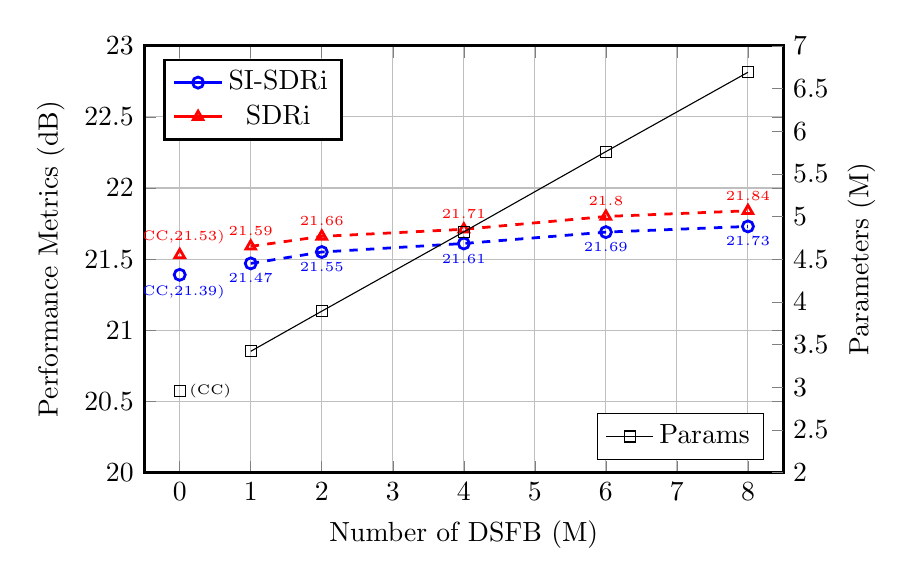
\begin{tikzpicture}
        % 第一个轴:用于性能指标
        \begin{axis}[
            %title={Performance Comparison of Varying Numbers of DSFB (M) on WSJ0-2Mix Dataset},
            xlabel={Number of DSFB (M)},
            ylabel={Performance Metrics (dB)},
            xmin=-0.5, xmax=8.5,
            ymin=20, ymax=23,
            xtick={0,1,...,8},
            ytick={20,20.5,...,23},
            grid=both, % 显示主次网格线
            width=0.8\columnwidth,
            height=7cm,
            legend pos=north west,
            ymajorgrids=true, % 启用X轴主要网格线
            xmajorgrids=true,
            line width=1pt,
            mark size=2pt,
            every axis plot post/.append style={mark options={solid}},
            % nodes near coords, % 添加此行以显示坐标
            % every node near coord/.append style={font=\tiny, /pgf/number format/.cd, fixed, precision=1}, % 设置坐标标签样式和格式
             %  % 数据点标记边框为实线
            ]
            
            % % SC 方法的 SI-SDRi 数据点
            % \addplot[
            %     color=blue,
            %     mark=o,
            %     ]
            %     coordinates {
            %     (0,21.0)
            %     } node[anchor=west, pos=1] {(SC)}; % 在点的右边添加文本
            %     %\addlegendentry{SC: SI-SDRi}
            % % SC 方法的SDRi 数据点
            % \addplot[
            %     color=red,
            %     mark=triangle,
            %     ]
            %     coordinates {
            %     (0,21.2)
            %     } node[anchor=west, pos=1] {(SC)}; % 在点的右边添加文本
            %     %\addlegendentry{SC: SI-SDRi}
            % % CC 方法的 SI-SDRi 数据点
            \addplot[
                color=blue,
                mark=o,
                ]
                coordinates {
                (0,21.39)
                } node[anchor=north, pos=1, font=\tiny] {(CC,21.39)};
               % \addlegendentry{CC: SI-SDRi}
            % CC 方法的 SDRi 数据点
            \addplot[
                color=red,
                mark=triangle,
                ]
                coordinates {
                (0,21.53)
                } node[anchor=south, pos=1, font=\tiny] {(CC,21.53)}; % 使用 \tiny 设置字体大小
               % \addlegendentry{CC: SI-SDRi}
                
            % DFC-Net 不同 M 值的 SI-SDRi 和 SDRi 数据点
            \addplot[
                color=blue,
                dashed,
                mark=o,
                nodes near coords, % 显示坐标
                every node near coord/.append style={
                    font=\tiny,
                    /pgf/number format/.cd, fixed, precision=2,
                },
                 nodes near coords align={below}, % 确保标签在下方
                ]
                coordinates {
                (1,21.47)(2,21.55)(4,21.61)(6,21.69)(8,21.73)
                };
                
                \addlegendentry{SI-SDRi}
                
            \addplot[
                color=red,
                dashed,
                mark=triangle,
                nodes near coords, % 显示坐标
                every node near coord/.append style={
                    font=\tiny,
                    /pgf/number format/.cd, fixed, precision=2,
                },
                nodes near coords align={above}, % 确保标签在上方
                ]
                coordinates {
                (1,21.59)(2,21.66)(4,21.71)(6,21.80)(8,21.84)
                };
                \addlegendentry{SDRi}
                
        \end{axis}
        
        % 第二个轴:用于参数量 Params(M)
        \begin{axis}[
            axis y line*=right,
            axis x line=none, % 隐藏第二个轴的X轴线
            ylabel={Parameters (M)},
            xmin=-0.5, xmax=8.5, % 保持与第一个轴相同的X轴范围
            ymin=2, ymax=7,
            ytick={2,2.5,...,7},
            % yticklabels={2.95,3.42,3.89,4.82,5.76,6.69},
            width=0.8\columnwidth,
            height=7cm,
            legend pos=south east,
            ]
            
            % Params(M) 数据点
            \addplot[
                color=black,
                mark=none,
                mark=square,
                ]
                coordinates {
                (1,3.42)(2,3.89)(4,4.82)(6,5.76)(8,6.69)
                };
                \addlegendentry{Params}
                
            % 绘制 SC 和 CC 的参数量(可选)
            \addplot[
                color=black,
                %dashed,
                mark=square,
                ]
                coordinates {
                (0,2.95)
                }node[anchor=west, pos=1, font=\tiny] {(CC)};
                %\addlegendentry{SC/CC Params}
                
        \end{axis}
    \end{tikzpicture}
    \caption{Performance comparison of varying numbers of DSFB (O) on the WSJ0-2Mix dataset, including parameter(M) count.}
    \label{fig:performance_comparison_with_params}
\end{figure}


\begin{table}[h]
\centering
\caption{Comparison model with diferent network}
\label{tab:sota4}
\begin{adjustbox}{max width=0.8\columnwidth} % 缩放表格以适应单栏的一半宽度
\resizebox{\linewidth}{!}{
\begin{tabular}{|c|c|c|c|c|}
\hline
\textbf{Methods} & \textbf{Params(M)} & \textbf{SI-SDRi} & \textbf{SDRi} \\ \hline
DFC-Net(RNN) & 3.7M & 20.8 & 21.0  \\ 
DFC-Net(BT) & 3.8M & 21.3 & 21.5  \\ 
DFC-Net(IT) & 3.9M  & \textbf{21.6} & \textbf{21.7}  \\ \hline

\end{tabular}
}
\end{adjustbox}
\end{table}

%Table \ref{tab:sota4} presents the different domain of our model, in Time domain, we use 1D convolution as encoder and form 2D representations through segment, overlap and stack chunks. The Time domain model is suboptimal probably because the spectrogram in the frequency domain contains richer 2D representations than Time domain.
Table \ref{tab:sota4} presents the different extraction network, DFC-Net (RNN) means we replace dual path trasnformer with dual path RNN. The following two are employed with base transformer (BT) \cite{vaswani2017attention} and improved transformer (IT) \cite{chen2020dual}. As we can see, IT yields the most effective performance.


\section{Conclusion}

%A conclusion section is not required. Although a conclusion may review the main points of the paper, do not replicate the abstract as the conclusion. A conclusion might elaborate on the importance of the work or suggest applications and extensions.
In this work, we propose a T-F domain target speaker separation network DCF-Net, in which DualStream Fusion Block is introduced to capture the interactions between contextualized enrollment and mixture representation across both spatial and channel dimensions. Numerical results show DCF-Net could outperform existing methods over the benchmark datasets. Future work we will explore more effective channel attention instead of SE in DSFB, and design more useful extraction network.


\newpage
%\section*{References}

\bibliography{article,refs}
\bibliographystyle{IEEEtran}

\end{document}
